
\documentclass[11pt,a4paper]{article}

% ---------- Packages ----------
\usepackage[margin=1in]{geometry}
\usepackage{graphicx}
\usepackage{amsmath, amssymb, amsthm}
\usepackage{booktabs}
\usepackage{array}
\usepackage{enumitem}
\usepackage[hidelinks]{hyperref}
\usepackage{titlesec}

% Optional: tighter run-in paragraph/subparagraph spacing
\titlespacing*{\paragraph}{0pt}{1.25ex plus .5ex}{1em}
\titlespacing*{\subparagraph}{0pt}{1.0ex plus .5ex}{1em}

% ---------- Macros ----------
% Common Hamiltonian notation
\newcommand{\Hising}{H_{\mathrm{Ising}}}
\newcommand{\Htf}{H_{\mathrm{TF}}}
\newcommand{\Htot}{H=\Hising+\Htf}

% A small helper for nice math in tables
\newcommand{\NNZ}{\#\text{non-zero components}}

% Table column types
\newcolumntype{L}[1]{>{\raggedright\arraybackslash}p{#1}}
\newcolumntype{C}[1]{>{\centering\arraybackslash}p{#1}}

% ---------- Header ----------
\title{Scars of the Transverse Field Ising Model on Discrete Geometries (Polyhedra)}
\author{}
\date{\today}

\begin{document}
\maketitle

% ============================================================
% OVERALL PARAGRAPH (global statement for the whole note)
% ============================================================
\section*{Introduction}
We are studying scars of the simple Ising model on discrete geometries (polyhedra). Here, \emph{scars} are identified as special, sparser eigenstates of the Hamiltonian which are simultaneously eigenstates of the Ising term and of the transverse-field (TF) term separately; in addition, each such state is annihilated by exactly one of the two terms. In all of the following examples, the Hamiltonian is

\begin{equation}
\Htot, \quad \Hising = J \sum_{\langle i,j\rangle} \sigma_i^x \sigma_j^x, \quad  \Htf = - h \sum_i \sigma_i^z
\end{equation}

where $J=1, h=3$ (antiferromagnetic, non critical).

\section*{Platonic Solids}
% ============================================================
% REPEAT THE BLOCK BELOW FOR EACH POLYHEDRON
% ============================================================

% -------------------- Polyhedron Block: START --------------------
\subsection*{Tetrahedron}

\subsubsection*{Overview and data}
\begin{center}
  % Put your graphic at the very beginning of the subparagraph
  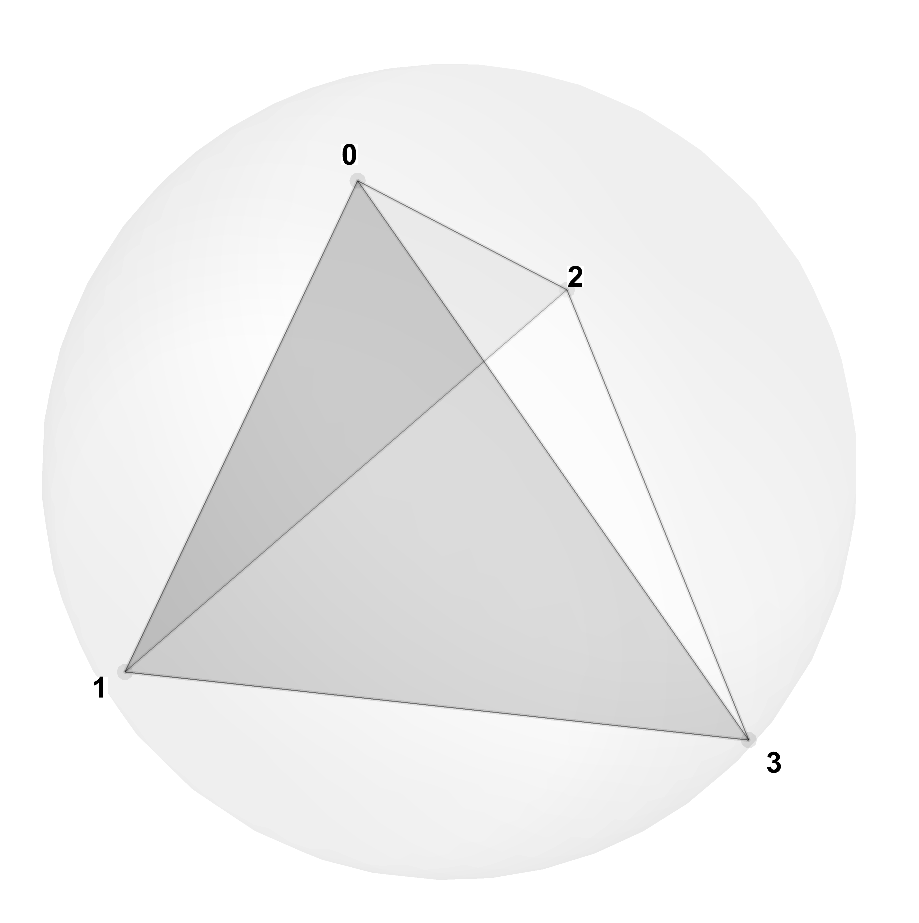
\includegraphics[width=.6\linewidth]{tetrahedron}
\end{center}

\begin{itemize}[leftmargin=1.5em]
  \item \textbf{Duality / paired solid:} self-dual, tetrahedron
  \item \textbf{Vertices (V), Faces (F), Edges (E):} $V = 4$,\; $F = 3$ (equilateral triangles),\; $E = 6$
  \item \textbf{Solid point group:} $T_d$\\
        \textbf{Vertex stabilizer subgroup:} $C_3$ for rotations only, $D_3$ for full symmetry group
  \item \textbf{Hilbert space:} \(
        \dim\mathcal{H} = 2^{4} = 16\ \text{(spin-$\tfrac12$ on each vertex)}
        \)
  \item \textbf{Eigenvalue range:} $[-12.37, 12.71]$
\end{itemize}

\subsubsection*{Scar structure: sets and multiplets}

\begin{itemize}[leftmargin=1.5em]
  \item \textbf{Number of scar sets:} 1
  \end{itemize}
  \hspace{6mm}For each scar set $S_k$:\\

\begin{center}
\begin{tabular}{L{3.5cm} C{2.2cm} C{2.2cm} C{2.2cm} C{3.0cm} C{3.2cm}}
\toprule
\textbf{Multiplet label} & \textbf{Energy $E$} & \textbf{Degeneracy} & \textbf{Annihilated by} & \textbf{Non-zero components (vs.\ $2^{4} = 16$)} \\
\midrule
$S_1$ & -2 & 2 & $\Htf$ & 4,6 \\
\bottomrule
\end{tabular}
\end{center}

\subsubsection*{Local properties (RDMs)}

\begin{itemize}[leftmargin=1.5em]
  \item \textbf{Local RDM definition:} $\rho_A=\mathrm{Tr}_{\bar A}(|\psi\rangle\langle\psi|)$ on compact subsets of $n=1$ sites, with $n < V/2, (V = 4)$
  \item \textbf{Compactness criterion:} NA, the single point ${0}$ was chosen
  \item \textbf{Diagnostics:} 1-site RDMs for both scars are full rank (system size $V=4$ is too small)
\end{itemize}

% -------------------- Polyhedron Block: END --------------------

% -------------------- Polyhedron Block: START --------------------
\subsection*{Octahedron}

\subsubsection*{Overview and data}
\begin{center}
  % Put your graphic at the very beginning of the subparagraph
  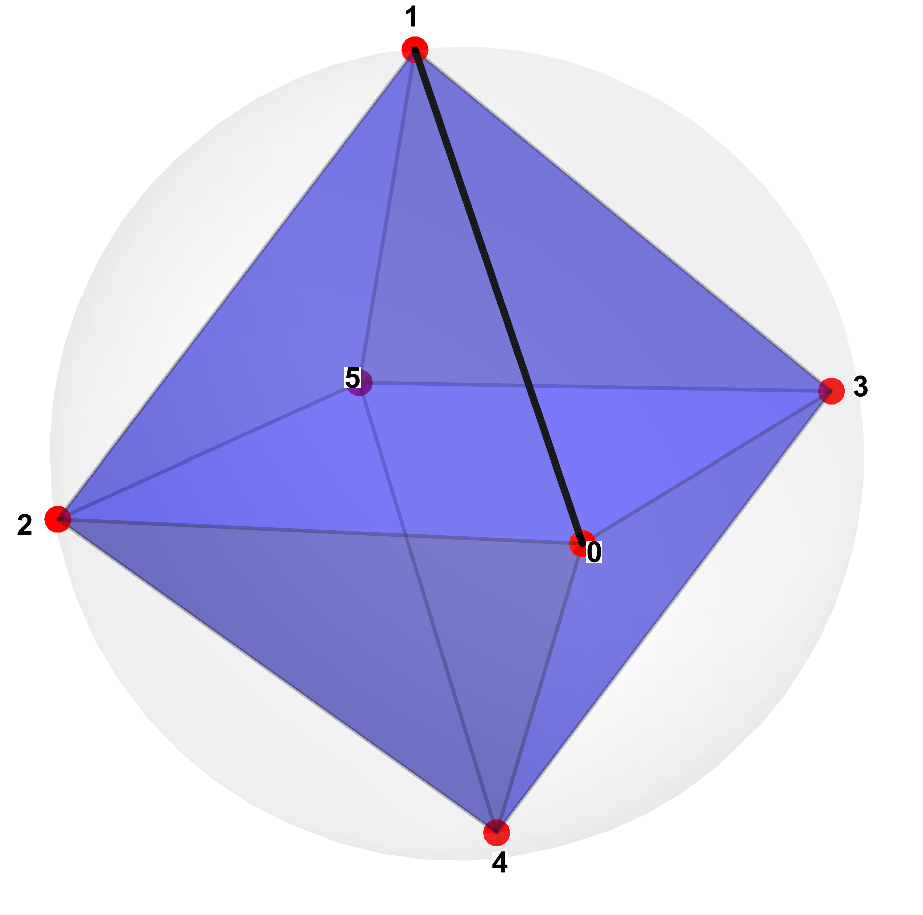
\includegraphics[width=.6\linewidth]{octahedron}
\end{center}

\begin{itemize}[leftmargin=1.5em]
  \item \textbf{Duality / paired solid:} cube
  \item \textbf{Vertices (V), Faces (F), Edges (E):} $V = 6$,\; $F = 8$ (equilateral triangles),\; $E = 12$
  \item \textbf{Solid point group:} $O_h$\\
        \textbf{Vertex stabilizer subgroup:} $C_4$ for rotations only, $C_{4v}$ for full symmetry group
  \item \textbf{Hilbert space:} \(
        \dim\mathcal{H} = 2^{6} = 64\ \text{(spin-$\tfrac12$ on each vertex)}
        \)
  \item \textbf{Eigenvalue range:} $[-18.80, 19.67]$
\end{itemize}

\subsubsection*{Scar structure: sets and multiplets}

\begin{itemize}[leftmargin=1.5em]
  \item \textbf{Number of scar sets:} 3
  \end{itemize}
  \hspace{6mm}For each scar set $S_k$:\\

\begin{center}
\begin{tabular}{L{3.5cm} C{2.2cm} C{2.2cm} C{2.2cm} C{3.0cm} C{3.2cm}}
\toprule
\textbf{Multiplet label} & \textbf{Energy $E$} & \textbf{Degeneracy} & \textbf{Annihilated by} & \textbf{Non-zero components (vs.\ $2^{6} = 64$)} \\
\midrule
$S_1$ & -6 & 3  & $\Hising$ & 12 \\
\midrule
$S_2$ & -4 & 1 & $\Htf$ & 12 \\
\midrule
$S_3$ & 6 & 3 & $\Hising$ & 12 \\
\bottomrule
\end{tabular}
\end{center}

\subsubsection*{Local properties (RDMs)}

\begin{itemize}[leftmargin=1.5em]
  \item \textbf{Local RDM definition:} $\rho_A=\mathrm{Tr}_{\bar A}(|\psi\rangle\langle\psi|)$ on compact subsets of $n=2$ sites, with $n < V/2, (V=6)$
  \item \textbf{Compactness criterion:} nearest-neighbor, for example $[0,1]$
   \item \textbf{Diagnostics:} 2-sites RDMs for all 7 scars are full rank (system size $V=6$ is too small)
\end{itemize}

% -------------------- Polyhedron Block: END --------------------

% -------------------- Polyhedron Block: START --------------------
\subsection*{Cube}

\subsubsection*{Overview and data}
\begin{center}
  % Put your graphic at the very beginning of the subparagraph
  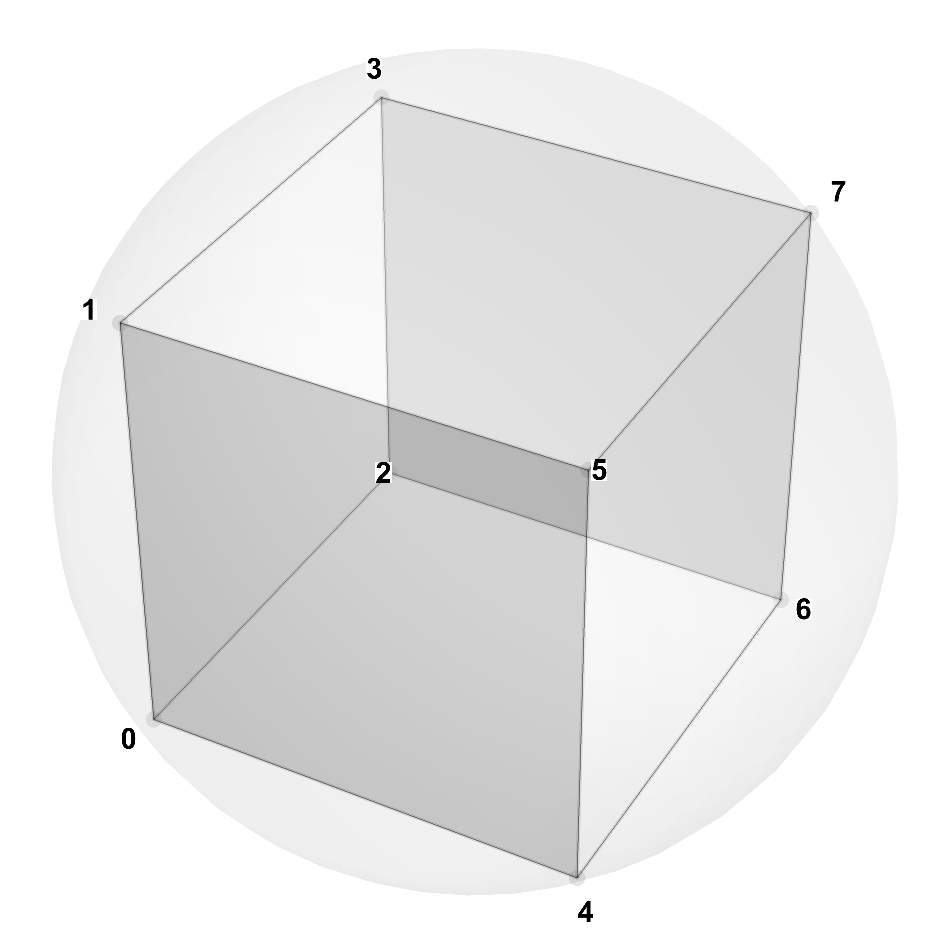
\includegraphics[width=.6\linewidth]{cube}
\end{center}

\begin{itemize}[leftmargin=1.5em]
  \item \textbf{Duality / paired solid:} octahedron
  \item \textbf{Vertices (V), Faces (F), Edges (E):} $V = 8$,\; $F = 6$ (squares),\; $E = 12$
  \item \textbf{Solid point group:} $O_h$\\
        \textbf{Vertex stabilizer subgroup:} $C_3$ for rotations only, $C_{3v}$ for full symmetry group
  \item \textbf{Hilbert space:} \(
        \dim\mathcal{H} = 2^{8} = 256\ \text{(spin-$\tfrac12$ on each vertex)}
        \)
  \item \textbf{Eigenvalue range:} $[-25.11, 25.11]$
\end{itemize}

\subsubsection*{Scar structure: sets and multiplets}

\begin{itemize}[leftmargin=1.5em]
  \item \textbf{Number of scar sets:} 2
  \end{itemize}
  \hspace{6mm}For each scar set $S_k$:\\

\begin{center}
\begin{tabular}{L{3.5cm} C{2.2cm} C{2.2cm} C{2.2cm} C{3.0cm} C{3.2cm}}
\toprule
\textbf{Multiplet label} & \textbf{Energy $E$} & \textbf{Degeneracy} & \textbf{Annihilated by} & \textbf{Non-zero components (vs.\ $2^{8} = 256$)} \\
\midrule
$S_1$ & -2 & 3 & $\Htf$ & 48 \\
\midrule
$S_2$ & 2 & 3 & $\Htf$ & 48 \\
\bottomrule
\end{tabular}
\end{center}

\subsubsection*{Local properties (RDMs)}

\begin{itemize}[leftmargin=1.5em]
  \item \textbf{Local RDM definition:} $\rho_A=\mathrm{Tr}_{\bar A}(|\psi\rangle\langle\psi|)$ on compact subsets of $n=2,3$ sites, with $n < V/2, (V = 8)$
  \item \textbf{Compactness criterion:} nearest-neighbor + most compact, for example $[0,1], [0,1,2]$
  \item \textbf{Diagnostics:} 2-sites RDMs for all 6 scars are full rank (system size $V=8$ is too small)
\end{itemize}

% -------------------- Polyhedron Block: END --------------------

% -------------------- Polyhedron Block: START --------------------
\subsection*{Icosahedron}

\subsubsection*{Overview and data}
\begin{center}
  % Put your graphic at the very beginning of the subparagraph
  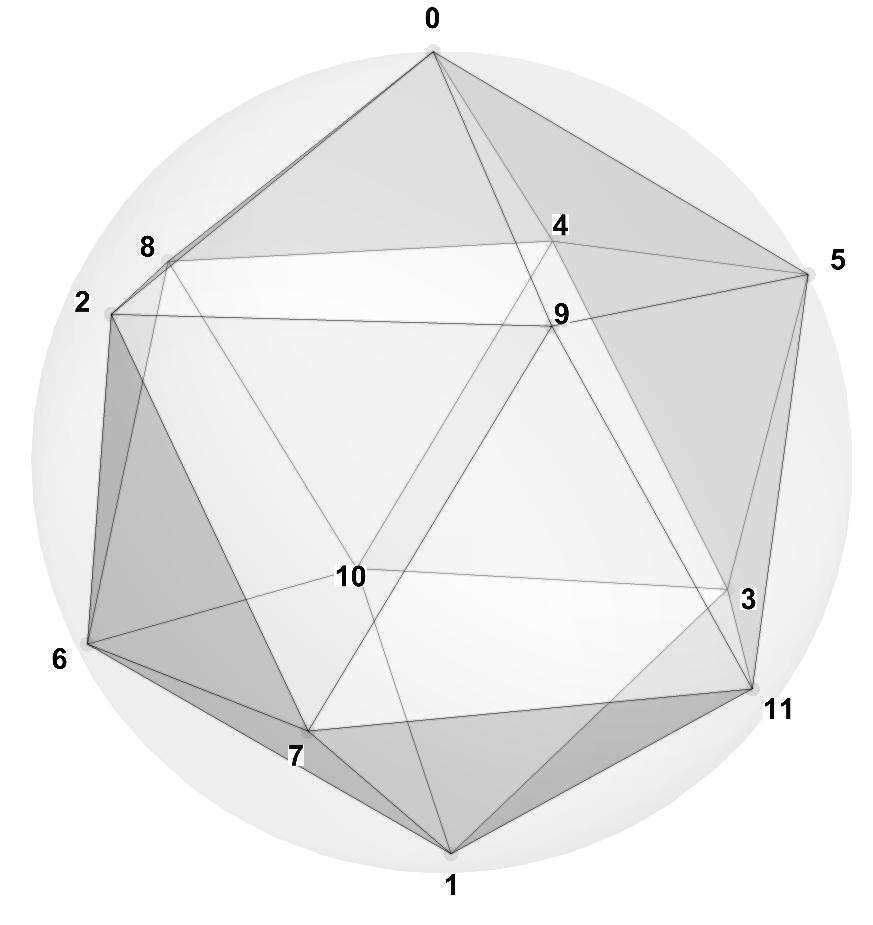
\includegraphics[width=.6\linewidth]{icosahedron}
\end{center}

\begin{itemize}[leftmargin=1.5em]
  \item \textbf{Duality / paired solid:} dodecahedron
  \item \textbf{Vertices (V), Faces (F), Edges (E):} $V = 12$,\; $F = 20$ (equilateral triangles),\; $E = 30$
  \item \textbf{Solid point group:} $I_h$\\
        \textbf{Vertex stabilizer subgroup:} $C_5$ for rotations only, $D_5$ for full symmetry group
  \item \textbf{Hilbert space:} \(
        \dim\mathcal{H} = 2^{12} = 4096\ \text{(spin-$\tfrac12$ on each vertex)}
        \)
  \item \textbf{Eigenvalue range:} $[-37.95, 41.29]$
\end{itemize}

\subsubsection*{Scar structure: sets and multiplets}

\begin{itemize}[leftmargin=1.5em]
  \item \textbf{Number of scar sets:} 1
  \end{itemize}
  \hspace{6mm}For each scar set $S_k$:\\

\begin{center}
\begin{tabular}{L{3.5cm} C{2.2cm} C{2.2cm} C{2.2cm} C{3.0cm} C{3.2cm}}
\toprule
\textbf{Multiplet label} & \textbf{Energy $E$} & \textbf{Degeneracy} & \textbf{Annihilated by} & \textbf{Non-zero components (vs.\ $2^{12} = 4096$)} \\
\midrule
$S_1$ & -6 & 5 & $\Htf$ & 280 \\
\bottomrule
\end{tabular}
\end{center}

\subsubsection*{Local properties (RDMs)}

\begin{itemize}[leftmargin=1.5em]
  \item \textbf{Local RDM definition:} $\rho_A=\mathrm{Tr}_{\bar A}(|\psi\rangle\langle\psi|)$ on compact subsets of $n=2,3,4,5$ sites, with $n < V/2, (V=12)$.
  \item \textbf{Compactness criterion:} \texttt{<how subsets chosen>}.
  \item \textbf{Diagnostics:} \begin{itemize} \item 2/3-sites RDMs for all 5 scars are full rank \item 4-sites RDMs for all 5 scars have reduced rank of 11 = 16 - 5 \item 5-sites RDMs for all 5 scars have reduced rank of 18 = 32 - 14 \end{itemize}
\end{itemize}

% -------------------- Polyhedron Block: END --------------------

% -------------------- Polyhedron Block: START --------------------
\subsection*{Dodecahedron}

\subsubsection*{Overview and data}
\begin{center}
  % Put your graphic at the very beginning of the subparagraph
  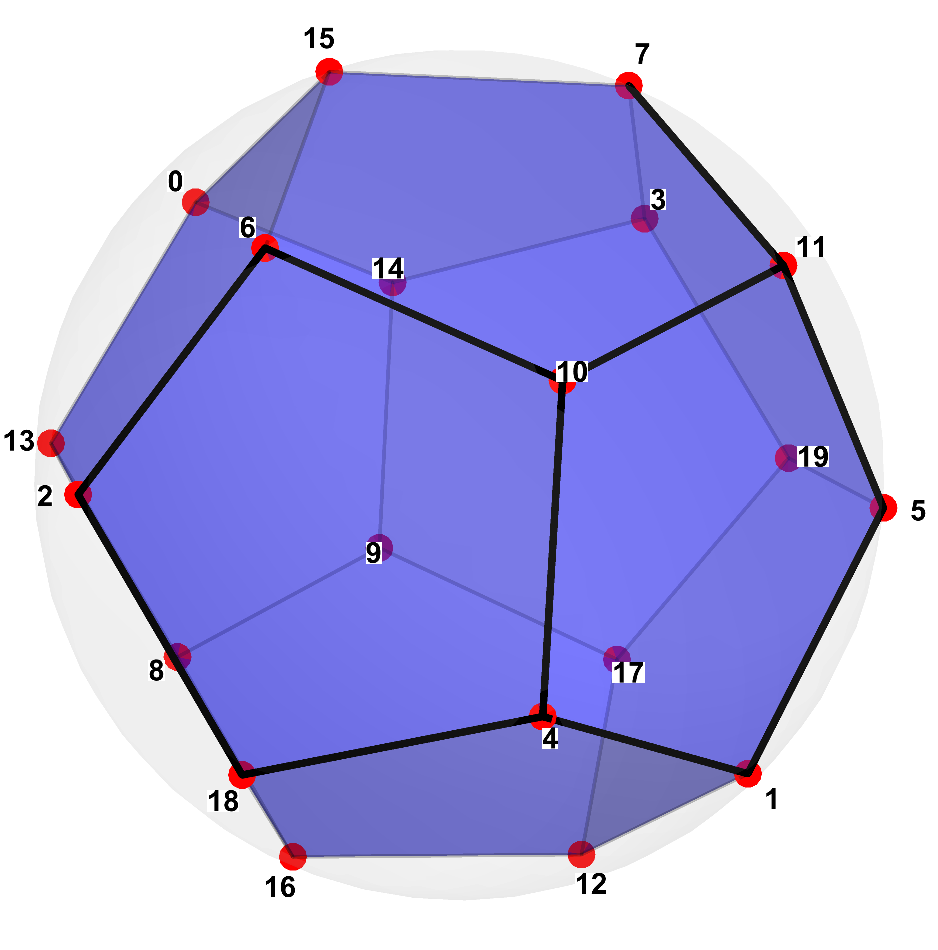
\includegraphics[width=.6\linewidth]{dodecahedron}
\end{center}

\begin{itemize}[leftmargin=1.5em]
  \item \textbf{Duality / paired solid:} icosahedron
  \item \textbf{Vertices (V), Faces (F), Edges (E):} $V = 20$,\; $F = 12$ (equilateral triangles),\; $E = 30$
  \item \textbf{Solid point group:} $I_h$\\
        \textbf{Vertex stabilizer subgroup:} $C_3$ for rotations only, $D_3$ for full symmetry group
  \item \textbf{Hilbert space:} \(
        \dim\mathcal{H} = 2^{20} = 1,048,576\ \text{(spin-$\tfrac12$ on each vertex)}
        \)
  \item \textbf{Eigenvalue range:} $[-12.37, 12.71]$
\end{itemize}

\subsubsection*{Scar structure: sets and multiplets}

\begin{itemize}[leftmargin=1.5em]
  \item \textbf{Number of scar sets:} 1
  \end{itemize}
  \hspace{6mm}For each scar set $S_k$:\\

\begin{center}
\begin{tabular}{L{3.5cm} C{2.2cm} C{2.2cm} C{2.2cm} C{3.0cm} C{3.2cm}}
\toprule
\textbf{Multiplet label} & \textbf{Energy $E$} & \textbf{Degeneracy} & \textbf{Annihilated by} & \textbf{Non-zero components (vs.\ $2^{20} = 1,048,576$)} \\
\midrule
$S_1$ & $\pm$ \texttt{<int>} & \texttt{<deg>} & \texttt{$\Hising$ / $\Htf$ / both} & \texttt{<\# non-zero> / $2^{\texttt{<V>}}$} \\
\bottomrule
\end{tabular}
\end{center}

\subsubsection*{Local properties (RDMs).}

\begin{itemize}[leftmargin=1.5em]
  \item \textbf{Local RDM definition:} $\rho_A=\mathrm{Tr}_{\bar A}(|\psi\rangle\langle\psi|)$ on compact subsets of $n=2,3,4,5,6,7,8,9$ sites, with $n < V/2, (V=20)$.
  \item \textbf{Compactness criterion:} \texttt{<how subsets chosen>}.
  \item \textbf{Diagnostics:} \texttt{<observables, entropies, purity, etc.>}.
\end{itemize}

% -------------------- Polyhedron Block: END --------------------

\section*{Catalan Solids}
% ============================================================
% REPEAT THE BLOCK BELOW FOR EACH POLYHEDRON
% ============================================================

% -------------------- Polyhedron Block: START --------------------
\subsection*{Triakis Tetrahedron}

\subsubsection*{Overview and data}
\begin{center}
  % Put your graphic at the very beginning of the subparagraph
  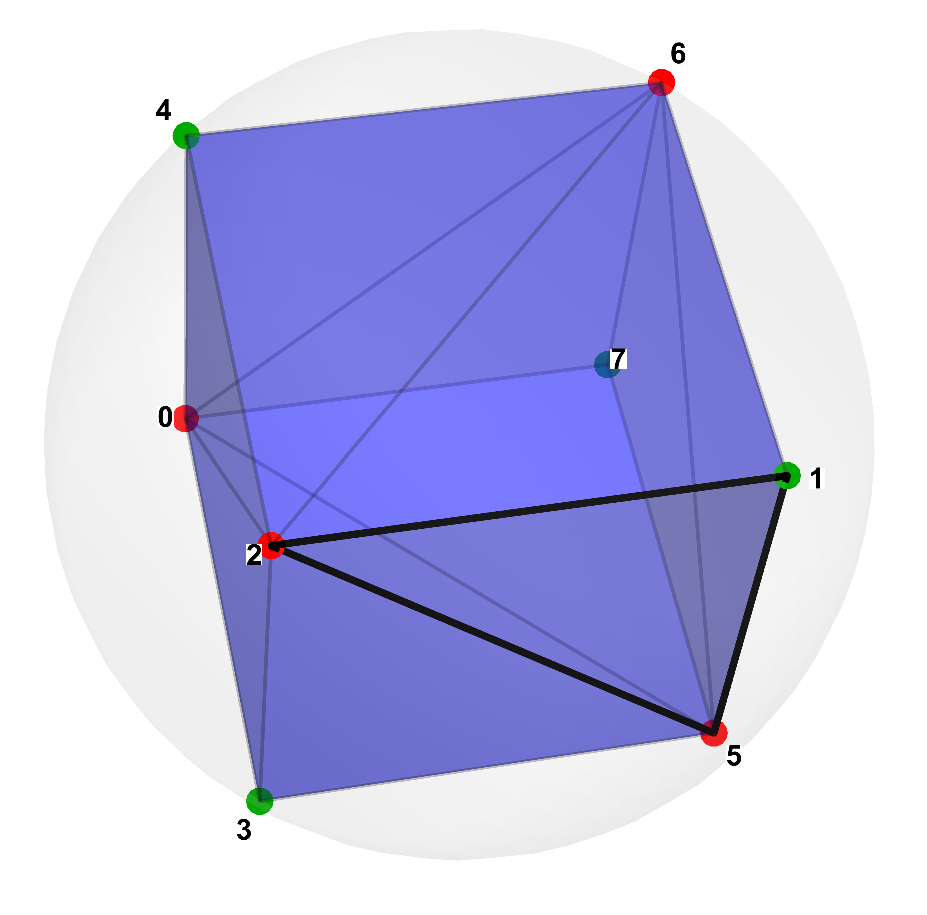
\includegraphics[width=.6\linewidth]{triakistetrahedron}
\end{center}

\begin{itemize}[leftmargin=1.5em]
  \item \textbf{Duality / paired solid:} self-dual, tetrahedron
  \item \textbf{Vertices (V), Faces (F), Edges (E):} $V = 4$,\; $F = 3$ (equilateral triangles),\; $E = 6$
  \item \textbf{Solid point group:} $T_d \cong S_4$\\
        \textbf{Vertex stabilizer subgroup:} $C_3$ for rotations only, $D_3$ for full symmetry group
  \item \textbf{Hilbert space:} \(
        \dim\mathcal{H} = 2^{4} = 16\ \text{(spin-$\tfrac12$ on each vertex)}
        \)
  \item \textbf{Eigenvalue range:} $[-12.37, 12.71]$
\end{itemize}

\subsubsection*{Scar structure: sets and multiplets}

\begin{itemize}[leftmargin=1.5em]
  \item \textbf{Number of scar sets:} 2
  \end{itemize}
  \hspace{6mm}For each scar set $S_k$:\\

\begin{center}
\begin{tabular}{L{3.5cm} C{2.2cm} C{2.2cm} C{2.2cm} C{3.0cm} C{3.2cm}}
\toprule
\textbf{Multiplet label} & \textbf{Energy $E$} & \textbf{Degeneracy} & \textbf{Annihilated by} & \textbf{Non-zero components (vs.\ $2^{V}$)} \\
\midrule
$S_1$ & $\pm$ \texttt{<int>} & \texttt{<deg>} & \texttt{$\Hising$ / $\Htf$ / both} & \texttt{<\# non-zero> / $2^{\texttt{<V>}}$} \\
\midrule
$S_2$ & $\pm$ \texttt{<int>} & \texttt{<deg>} & \texttt{$\Hising$ / $\Htf$ / both} & \texttt{<\# non-zero> / $2^{\texttt{<V>}}$} \\
\bottomrule
\end{tabular}
\end{center}

\subsubsection*{Local properties (RDMs).}

\begin{itemize}[leftmargin=1.5em]
  \item \textbf{Local RDM definition:} $\rho_A=\mathrm{Tr}_{\bar A}(|\psi\rangle\langle\psi|)$ on compact subsets of $n=2,3,4,5,6$ sites, with $n < V/2$.
  \item \textbf{Compactness criterion:} \texttt{<how subsets chosen>}.
  \item \textbf{Diagnostics:} \texttt{<observables, entropies, purity, etc.>}.
\end{itemize}

% -------------------- Polyhedron Block: END ---------------------

% -------------------- Polyhedron Block: START --------------------
\subsection*{Rhombic Dodecahedron}

\subsubsection*{Overview and data}
\begin{center}
  % Put your graphic at the very beginning of the subparagraph
  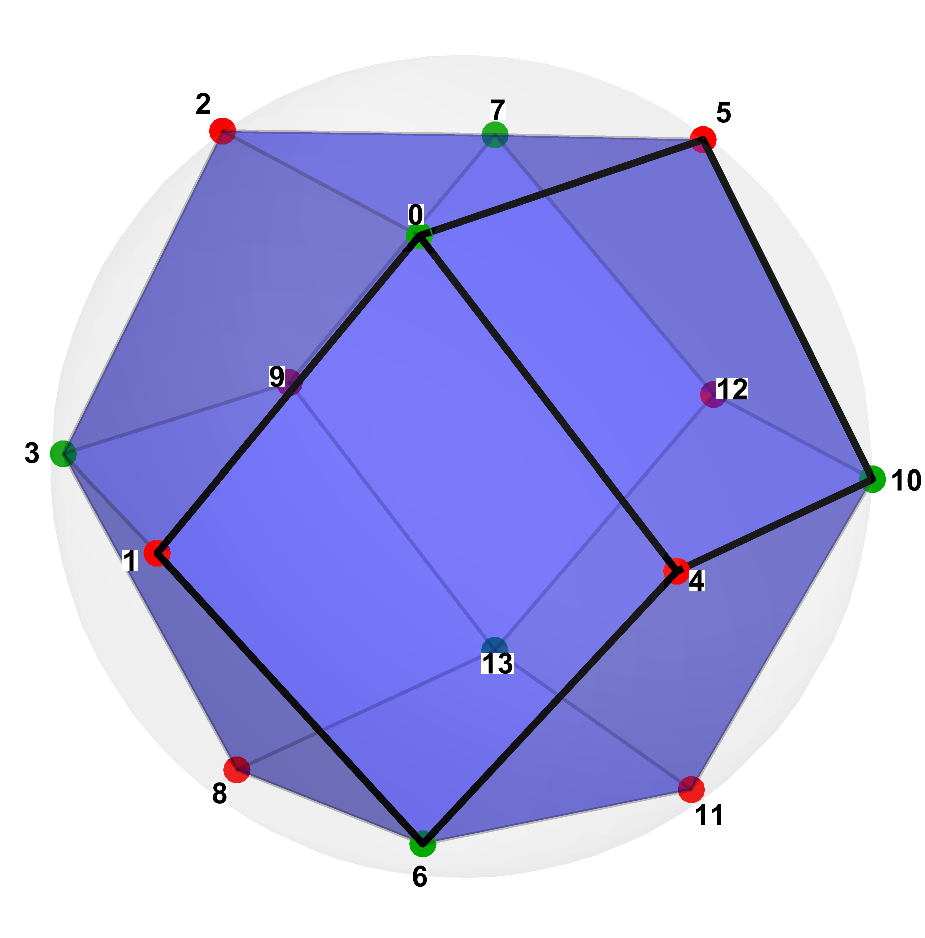
\includegraphics[width=.6\linewidth]{rhombicdodecahedron}
\end{center}

\begin{itemize}[leftmargin=1.5em]
  \item \textbf{Duality / paired solid:} self-dual, tetrahedron
  \item \textbf{Vertices (V), Faces (F), Edges (E):} $V = 4$,\; $F = 3$ (equilateral triangles),\; $E = 6$
  \item \textbf{Solid point group:} $T_d \cong S_4$\\
        \textbf{Vertex stabilizer subgroup:} $C_3$ for rotations only, $D_3$ for full symmetry group
  \item \textbf{Hilbert space:} \(
        \dim\mathcal{H} = 2^{4} = 16\ \text{(spin-$\tfrac12$ on each vertex)}
        \)
  \item \textbf{Eigenvalue range:} $[-12.37, 12.71]$
\end{itemize}

\subsubsection*{Scar structure: sets and multiplets}

\begin{itemize}[leftmargin=1.5em]
  \item \textbf{Number of scar sets:} 2
  \end{itemize}
  \hspace{6mm}For each scar set $S_k$:\\

\begin{center}
\begin{tabular}{L{3.5cm} C{2.2cm} C{2.2cm} C{2.2cm} C{3.0cm} C{3.2cm}}
\toprule
\textbf{Multiplet label} & \textbf{Energy $E$} & \textbf{Degeneracy} & \textbf{Annihilated by} & \textbf{Non-zero components (vs.\ $2^{V}$)} \\
\midrule
$S_1$ & $\pm$ \texttt{<int>} & \texttt{<deg>} & \texttt{$\Hising$ / $\Htf$ / both} & \texttt{<\# non-zero> / $2^{\texttt{<V>}}$} \\
\midrule
$S_2$ & $\pm$ \texttt{<int>} & \texttt{<deg>} & \texttt{$\Hising$ / $\Htf$ / both} & \texttt{<\# non-zero> / $2^{\texttt{<V>}}$} \\
\bottomrule
\end{tabular}
\end{center}

\subsubsection*{Local properties (RDMs).}

\begin{itemize}[leftmargin=1.5em]
  \item \textbf{Local RDM definition:} $\rho_A=\mathrm{Tr}_{\bar A}(|\psi\rangle\langle\psi|)$ on compact subsets of $n=2,3,4,5,6$ sites, with $n < V/2$.
  \item \textbf{Compactness criterion:} \texttt{<how subsets chosen>}.
  \item \textbf{Diagnostics:} \texttt{<observables, entropies, purity, etc.>}.
\end{itemize}

% -------------------- Polyhedron Block: END --------------------

% -------------------- Polyhedron Block: START --------------------
\subsection*{Triakis Octahedron}

\subsubsection*{Overview and data}
\begin{center}
  % Put your graphic at the very beginning of the subparagraph
  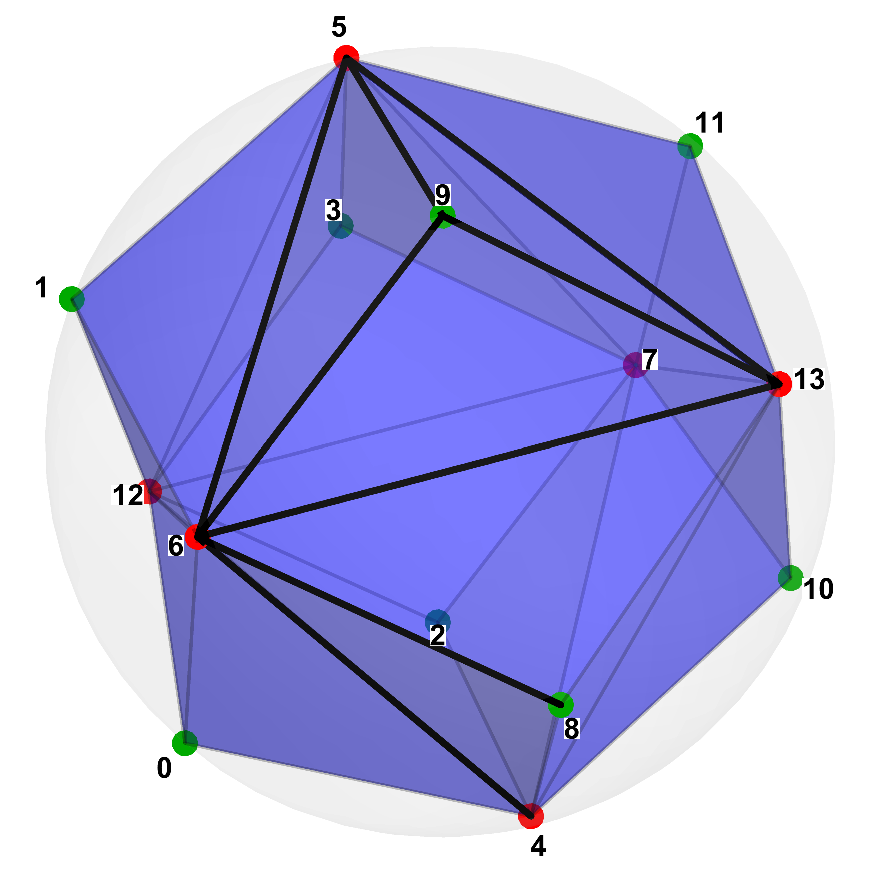
\includegraphics[width=.6\linewidth]{triakisoctahedron}
\end{center}

\begin{itemize}[leftmargin=1.5em]
  \item \textbf{Duality / paired solid:} self-dual, tetrahedron
  \item \textbf{Vertices (V), Faces (F), Edges (E):} $V = 4$,\; $F = 3$ (equilateral triangles),\; $E = 6$
  \item \textbf{Solid point group:} $T_d \cong S_4$\\
        \textbf{Vertex stabilizer subgroup:} $C_3$ for rotations only, $D_3$ for full symmetry group
  \item \textbf{Hilbert space:} \(
        \dim\mathcal{H} = 2^{4} = 16\ \text{(spin-$\tfrac12$ on each vertex)}
        \)
  \item \textbf{Eigenvalue range:} $[-12.37, 12.71]$
\end{itemize}

\subsubsection*{Scar structure: sets and multiplets}

\begin{itemize}[leftmargin=1.5em]
  \item \textbf{Number of scar sets:} 2
  \end{itemize}
  \hspace{6mm}For each scar set $S_k$:\\

\begin{center}
\begin{tabular}{L{3.5cm} C{2.2cm} C{2.2cm} C{2.2cm} C{3.0cm} C{3.2cm}}
\toprule
\textbf{Multiplet label} & \textbf{Energy $E$} & \textbf{Degeneracy} & \textbf{Annihilated by} & \textbf{Non-zero components (vs.\ $2^{V}$)} \\
\midrule
$S_1$ & $\pm$ \texttt{<int>} & \texttt{<deg>} & \texttt{$\Hising$ / $\Htf$ / both} & \texttt{<\# non-zero> / $2^{\texttt{<V>}}$} \\
\midrule
$S_2$ & $\pm$ \texttt{<int>} & \texttt{<deg>} & \texttt{$\Hising$ / $\Htf$ / both} & \texttt{<\# non-zero> / $2^{\texttt{<V>}}$} \\
\bottomrule
\end{tabular}
\end{center}

\subsubsection*{Local properties (RDMs).}

\begin{itemize}[leftmargin=1.5em]
  \item \textbf{Local RDM definition:} $\rho_A=\mathrm{Tr}_{\bar A}(|\psi\rangle\langle\psi|)$ on compact subsets of $n=2,3,4,5,6$ sites, with $n < V/2$.
  \item \textbf{Compactness criterion:} \texttt{<how subsets chosen>}.
  \item \textbf{Diagnostics:} \texttt{<observables, entropies, purity, etc.>}.
\end{itemize}

% -------------------- Polyhedron Block: END --------------------

% -------------------- Polyhedron Block: START --------------------
\subsection*{Tetrakis Hexahedron}

\subsubsection*{Overview and data.}\subsubsection*{Overview and data}
\begin{center}
  % Put your graphic at the very beginning of the subparagraph
  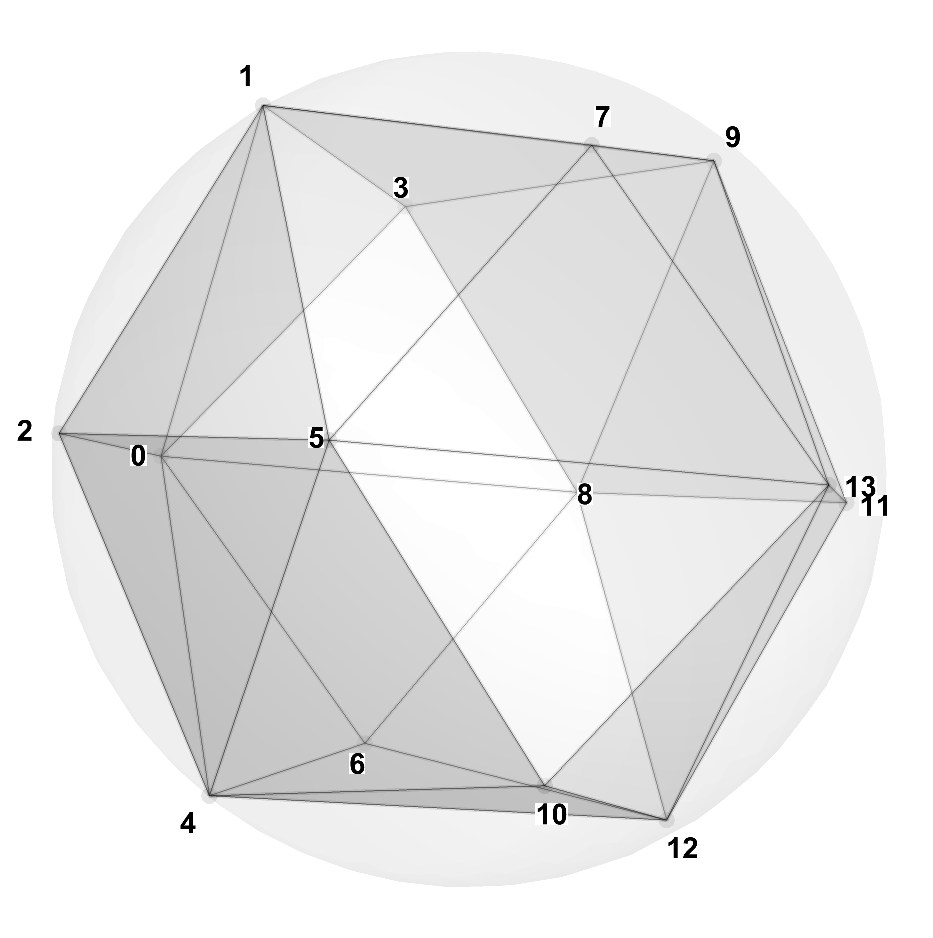
\includegraphics[width=.6\linewidth]{tetrakishexahedron}
\end{center}

\begin{itemize}[leftmargin=1.5em]
  \item \textbf{Duality / paired solid:} self-dual, tetrahedron
  \item \textbf{Vertices (V), Faces (F), Edges (E):} $V = 4$,\; $F = 3$ (equilateral triangles),\; $E = 6$
  \item \textbf{Solid point group:} $T_d \cong S_4$\\
        \textbf{Vertex stabilizer subgroup:} $C_3$ for rotations only, $D_3$ for full symmetry group
  \item \textbf{Hilbert space:} \(
        \dim\mathcal{H} = 2^{4} = 16\ \text{(spin-$\tfrac12$ on each vertex)}
        \)
  \item \textbf{Eigenvalue range:} $[-12.37, 12.71]$
\end{itemize}

\subsubsection*{Scar structure: sets and multiplets}

\begin{itemize}[leftmargin=1.5em]
  \item \textbf{Number of scar sets:} 2
  \end{itemize}
  \hspace{6mm}For each scar set $S_k$:\\

\begin{center}
\begin{tabular}{L{3.5cm} C{2.2cm} C{2.2cm} C{2.2cm} C{3.0cm} C{3.2cm}}
\toprule
\textbf{Multiplet label} & \textbf{Energy $E$} & \textbf{Degeneracy} & \textbf{Annihilated by} & \textbf{Non-zero components (vs.\ $2^{V}$)} \\
\midrule
$S_1$ & $\pm$ \texttt{<int>} & \texttt{<deg>} & \texttt{$\Hising$ / $\Htf$ / both} & \texttt{<\# non-zero> / $2^{\texttt{<V>}}$} \\
\midrule
$S_2$ & $\pm$ \texttt{<int>} & \texttt{<deg>} & \texttt{$\Hising$ / $\Htf$ / both} & \texttt{<\# non-zero> / $2^{\texttt{<V>}}$} \\
\bottomrule
\end{tabular}
\end{center}

\subsubsection*{Local properties (RDMs).}

\begin{itemize}[leftmargin=1.5em]
  \item \textbf{Local RDM definition:} $\rho_A=\mathrm{Tr}_{\bar A}(|\psi\rangle\langle\psi|)$ on compact subsets of $n=2,3,4,5,6$ sites, with $n < V/2$.
  \item \textbf{Compactness criterion:} \texttt{<how subsets chosen>}.
  \item \textbf{Diagnostics:} \texttt{<observables, entropies, purity, etc.>}.
\end{itemize}

% -------------------- Polyhedron Block: END --------------------


\section*{Archimedean Solids}
% ============================================================
% REPEAT THE BLOCK BELOW FOR EACH POLYHEDRON
% ============================================================

% -------------------- Polyhedron Block: START --------------------
\subsection*{Truncated Tetrahedron}

\subsubsection*{Overview and data}
\begin{center}
  % Put your graphic at the very beginning of the subparagraph
  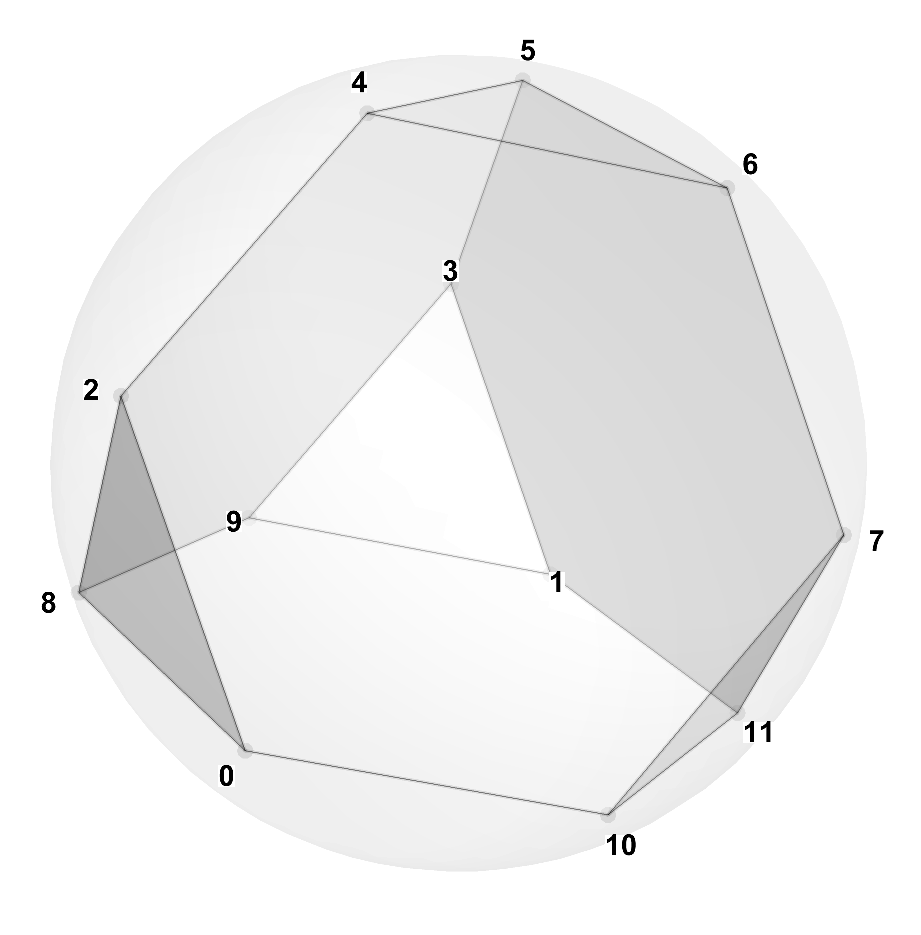
\includegraphics[width=.6\linewidth]{truncatedtetrahedron}
\end{center}

\begin{itemize}[leftmargin=1.5em]
  \item \textbf{Duality / paired solid:} self-dual, tetrahedron
  \item \textbf{Vertices (V), Faces (F), Edges (E):} $V = 4$,\; $F = 3$ (equilateral triangles),\; $E = 6$
  \item \textbf{Solid point group:} $T_d \cong S_4$\\
        \textbf{Vertex stabilizer subgroup:} $C_3$ for rotations only, $D_3$ for full symmetry group
  \item \textbf{Hilbert space:} \(
        \dim\mathcal{H} = 2^{4} = 16\ \text{(spin-$\tfrac12$ on each vertex)}
        \)
  \item \textbf{Eigenvalue range:} $[-12.37, 12.71]$
\end{itemize}

\subsubsection*{Scar structure: sets and multiplets}

\begin{itemize}[leftmargin=1.5em]
  \item \textbf{Number of scar sets:} 2
  \end{itemize}
  \hspace{6mm}For each scar set $S_k$:\\

\begin{center}
\begin{tabular}{L{3.5cm} C{2.2cm} C{2.2cm} C{2.2cm} C{3.0cm} C{3.2cm}}
\toprule
\textbf{Multiplet label} & \textbf{Energy $E$} & \textbf{Degeneracy} & \textbf{Annihilated by} & \textbf{Non-zero components (vs.\ $2^{V}$)} \\
\midrule
$S_1$ & $\pm$ \texttt{<int>} & \texttt{<deg>} & \texttt{$\Hising$ / $\Htf$ / both} & \texttt{<\# non-zero> / $2^{\texttt{<V>}}$} \\
\midrule
$S_2$ & $\pm$ \texttt{<int>} & \texttt{<deg>} & \texttt{$\Hising$ / $\Htf$ / both} & \texttt{<\# non-zero> / $2^{\texttt{<V>}}$} \\
\bottomrule
\end{tabular}
\end{center}

\subsubsection*{Local properties (RDMs).}

\begin{itemize}[leftmargin=1.5em]
  \item \textbf{Local RDM definition:} $\rho_A=\mathrm{Tr}_{\bar A}(|\psi\rangle\langle\psi|)$ on compact subsets of $n=2,3,4,5,6$ sites, with $n < V/2$.
  \item \textbf{Compactness criterion:} \texttt{<how subsets chosen>}.
  \item \textbf{Diagnostics:} \texttt{<observables, entropies, purity, etc.>}.
\end{itemize}

% -------------------- Polyhedron Block: END --------------------

% -------------------- Polyhedron Block: START --------------------
\subsection*{Cuboctahedron}

\subsubsection*{Overview and data}
\begin{center}
  % Put your graphic at the very beginning of the subparagraph
  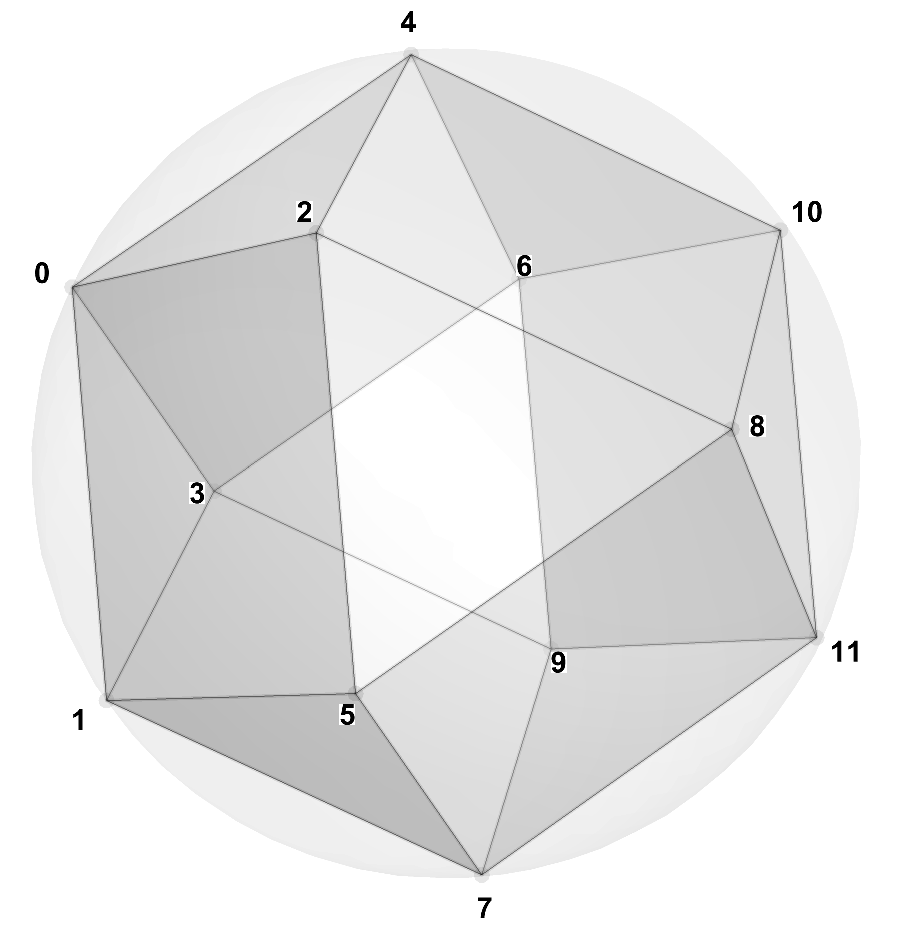
\includegraphics[width=.6\linewidth]{cuboctahedron}
\end{center}

\begin{itemize}[leftmargin=1.5em]
  \item \textbf{Duality / paired solid:} self-dual, tetrahedron
  \item \textbf{Vertices (V), Faces (F), Edges (E):} $V = 4$,\; $F = 3$ (equilateral triangles),\; $E = 6$
  \item \textbf{Solid point group:} $T_d \cong S_4$\\
        \textbf{Vertex stabilizer subgroup:} $C_3$ for rotations only, $D_3$ for full symmetry group
  \item \textbf{Hilbert space:} \(
        \dim\mathcal{H} = 2^{4} = 16\ \text{(spin-$\tfrac12$ on each vertex)}
        \)
  \item \textbf{Eigenvalue range:} $[-12.37, 12.71]$
\end{itemize}

\subsubsection*{Scar structure: sets and multiplets}

\begin{itemize}[leftmargin=1.5em]
  \item \textbf{Number of scar sets:} 2
  \end{itemize}
  \hspace{6mm}For each scar set $S_k$:\\

\begin{center}
\begin{tabular}{L{3.5cm} C{2.2cm} C{2.2cm} C{2.2cm} C{3.0cm} C{3.2cm}}
\toprule
\textbf{Multiplet label} & \textbf{Energy $E$} & \textbf{Degeneracy} & \textbf{Annihilated by} & \textbf{Non-zero components (vs.\ $2^{V}$)} \\
\midrule
$S_1$ & $\pm$ \texttt{<int>} & \texttt{<deg>} & \texttt{$\Hising$ / $\Htf$ / both} & \texttt{<\# non-zero> / $2^{\texttt{<V>}}$} \\
\midrule
$S_2$ & $\pm$ \texttt{<int>} & \texttt{<deg>} & \texttt{$\Hising$ / $\Htf$ / both} & \texttt{<\# non-zero> / $2^{\texttt{<V>}}$} \\
\bottomrule
\end{tabular}
\end{center}

\subsubsection*{Local properties (RDMs).}

\begin{itemize}[leftmargin=1.5em]
  \item \textbf{Local RDM definition:} $\rho_A=\mathrm{Tr}_{\bar A}(|\psi\rangle\langle\psi|)$ on compact subsets of $n=2,3,4,5,6$ sites, with $n < V/2$.
  \item \textbf{Compactness criterion:} \texttt{<how subsets chosen>}.
  \item \textbf{Diagnostics:} \texttt{<observables, entropies, purity, etc.>}.
\end{itemize}

% -------------------- Polyhedron Block: END --------------------

\paragraph*{Conclusions}
The eigenstates corresponding to eigenvalue 0, which are annihilated by both $\Hising$ and $\Htf$, are probably not proper scars, since they are not really sparse.

\end{document}
